Accurate full system simulators, with support for the latest hardware and its 
features are hugely complex, both for the developers and the users. The gem5 
simulator is definitely a powerful tool, but it unfortunately seems to be in a 
somewhat fragile and undocumented state concerning DVFS and power models at the 
moment.

Whilst the predictions done were not based on much data, it was demonstrated 
that predictions can be done and that even with little data, the predictions can
be very good. Changing the configurations was shown to affect the performance 
and energy consumption of the setups, sometimes drastically. This demonstrates 
the importance of managing the DVFS of cores and clusters, and that there is 
potentially a lot to be gained in terms of power savings. Based on the results 
from the predictions, the true optima, and the baselines, it seems schedulers 
should be able to use the PMUs to make informed decisions as to what silicon to 
keep dark in order to balance energy consumption and performance, although some 
attention will likely have to be paid to ensure the scale of performance and 
energy savings is balanced along with the values. Additionally, it seems that 
even a simple model can have a relatively high success rate. This could mean 
that PMU-aware schedulers could be implemented at a low performance cost, which 
is highly desirable for schedulers.
\begin{figure}[H]
    \centering
    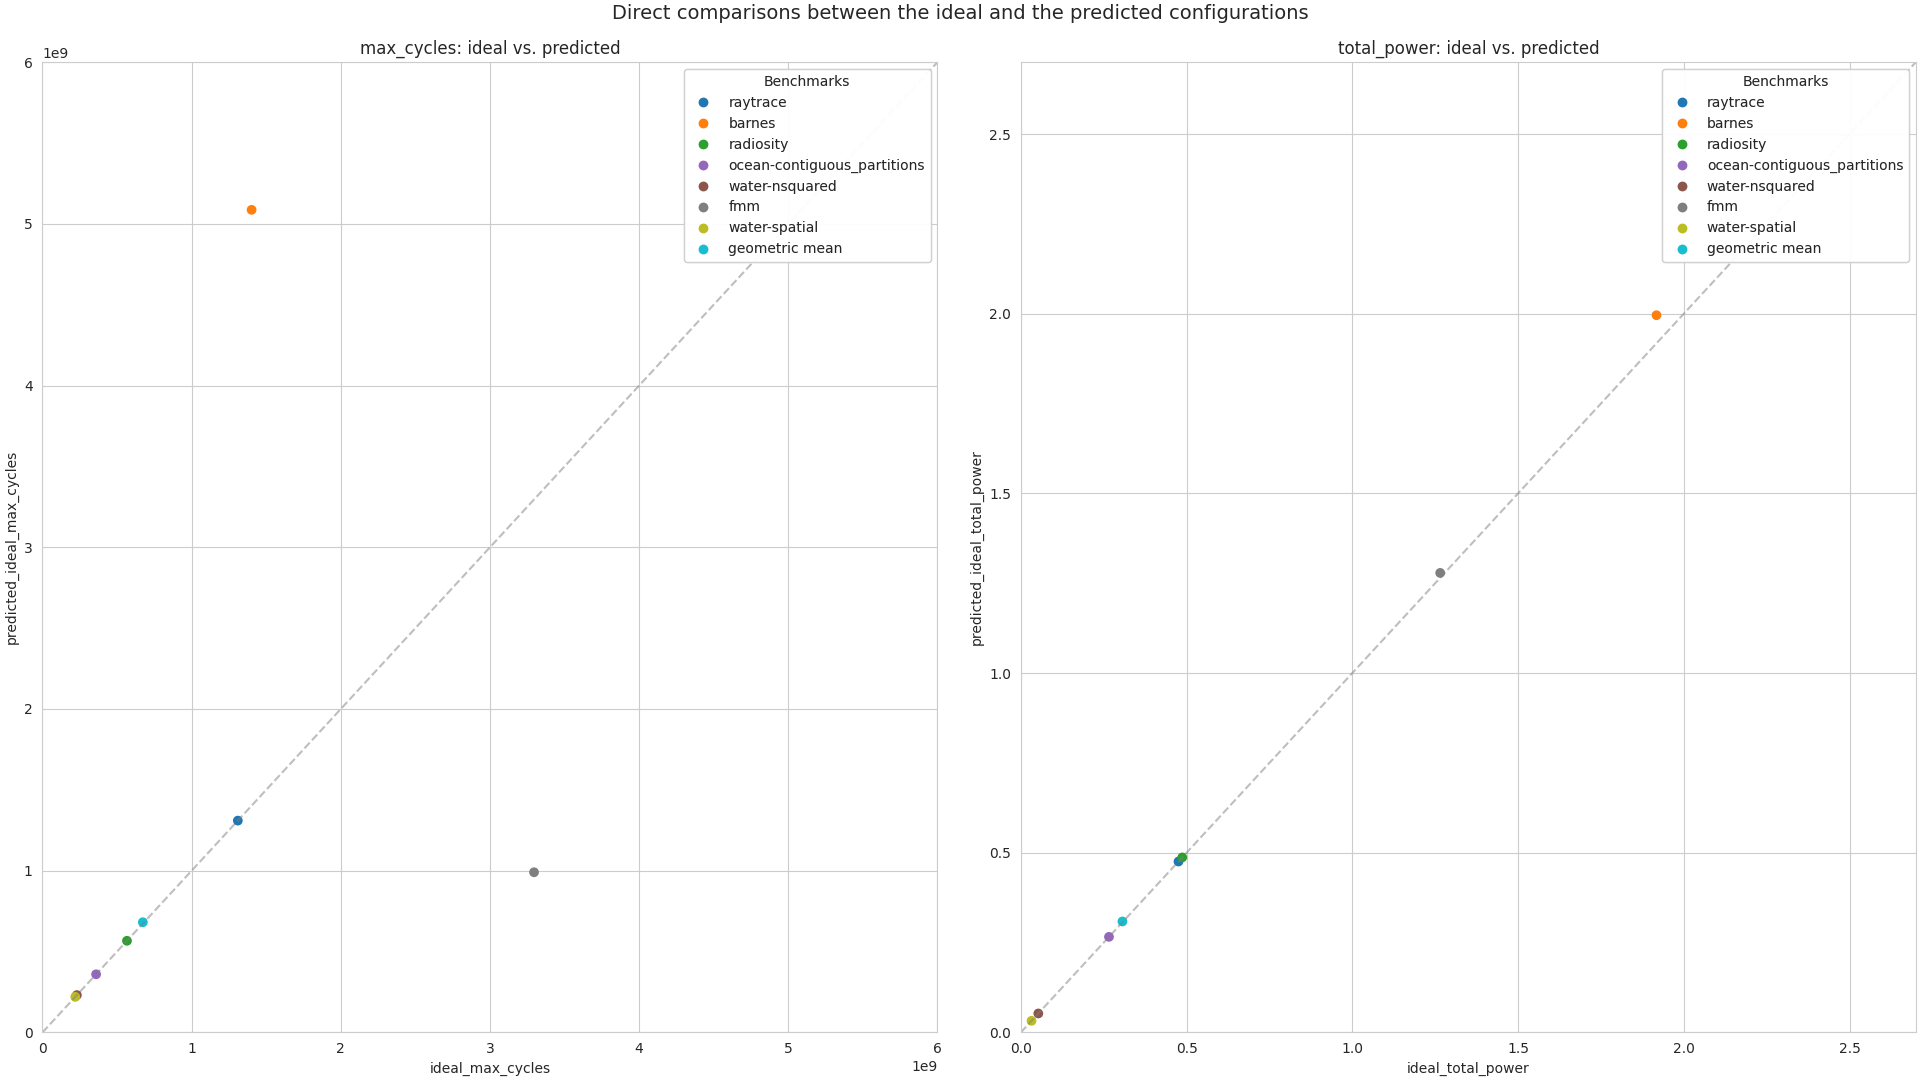
\includegraphics[width=0.7\textwidth]{result-plots/stock-2b2L/system-scatter.png}
    \caption{Even a simple model based on little data has a relatively good
             accuracy at predicting the best configurations}
\end{figure}

Given more time, I would have liked to get more data by also running 
configurations with only big or LITTLE cores and try to get the predictions to 
work for varying numbers of threads as well. Other future work could include 
the implementation on real hardware with multiple programs running 
simultaneously; improving the predictions by determining the feature importance 
of the different PMU events; playing with the balance of the optimum finder, to 
see if better optima could be found if power is prioritised over number of 
cycles, or vice versa. Although the initial results obtained in this project 
are based on a small sample size, they suggest that there is narrow space for 
improvement in terms of achieving the best performance, but also motivates the 
future work by demonstrating that even a relatively simple model trained on 
little data seems to produce this narrow optimisation space.
\begin{figure}[H]
    \centering
    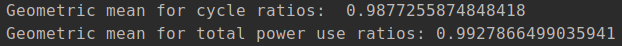
\includegraphics[width=0.6\textwidth]{screenshots/promising-geomeans.png}
    \caption{Although based on a small sample size, the model seems to have a
             narrow optimisation space}
\end{figure}
